\begin{frame}{Preprocessing}{How can we combine all the available data in a single set?}

\vspace{0.15cm}

    \emph{Raw} data sets has to be \textcolor{cyan}{cleaned}, and \emph{disaggregated data} can be \textcolor{cyan}{aggregated} to match the appropriate \emph{primary key}. \\

    \vspace{0.25cm}

    Then, they can be \alert{joined} --- for example, like this:

    \vspace{0.25cm}

    \begin{centering}
        \hspace*{-0.65cm}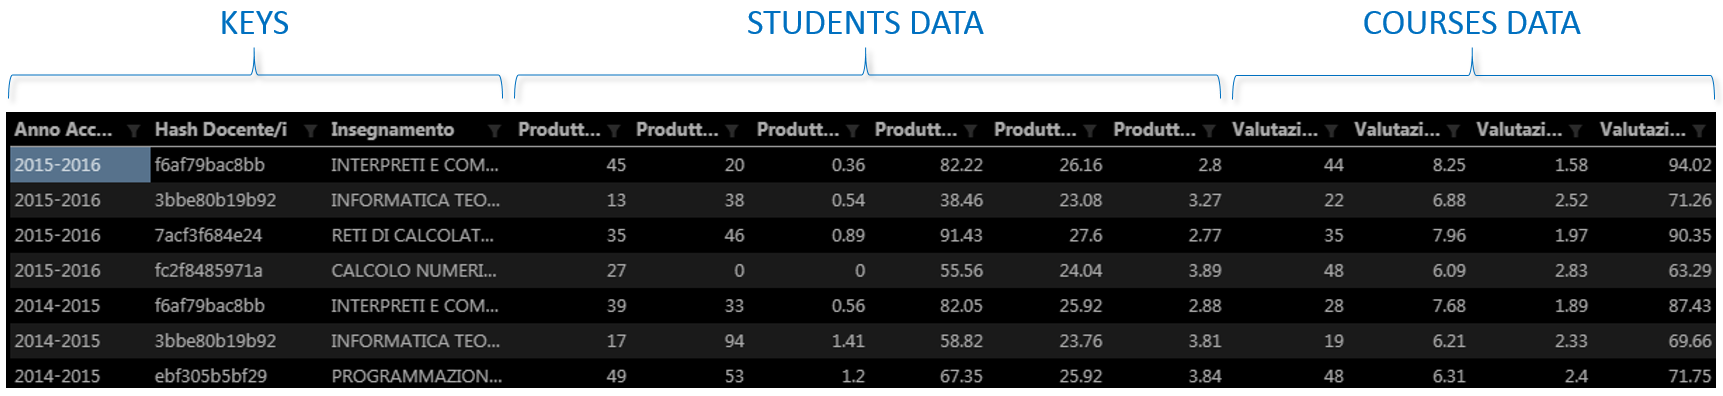
\includegraphics[scale=0.2]{prepr2.png}
    \end{centering}

\vspace{-0.35cm}
    Before attemping any data mining technique, data may still need \textcolor{cyan}{discretization}, \textcolor{cyan}{normalization}, etc. \\

 \vspace{0.25cm}

    Each analysis needs its own \emph{specific preprocessing}.

\end{frame}